%%%%%%%%%%%%%%%%%%%%%%%%%%%
% LaTeX package inclusion %
%%%%%%%%%%%%%%%%%%%%%%%%%%%
\usepackage{times}
\usepackage{units}
\usepackage{mathrsfs}
% \usepackage{diss} % defines \bv and some other stuff
\usepackage{subfigure}
\usepackage{multirow}
\usepackage{amsmath}
\usepackage{amssymb}
%\usepackage{movie15} % Do not use w/ multimedia
\usepackage{multimedia}
\usepackage{algorithm}
\usepackage{algorithmic}
%\usepackage{verbatim} % DO NOT include verbatim.  I think it messes up the semiverbatim environment!
\usepackage{booktabs}

% Package to include when making a handout.  You will probably need to install
% PGF before you can use these.  I did not yet find an RPM :-(
% Something seems to be wrong with this package.  It gives me a bunch of the following errors:
% Illegal unit of measure (pt inserted).
%\usepackage{pgf,pgfpages}
%\pgfpagesuselayout{4 on 1}[letterpaper,landscape,border shrink=0.5in]




% makes slide bg slightly gray in handouts, may help delineate slide boundaries
% Note that you can make acrobat print slide borders automatically as well...
%\mode<handout>{\setbeamercolor{background canvas}{bg=black!5}} 
\setlength{\fboxrule}{1pt} % Thicker boxes may help you in setting viewports
\setlength{\fboxsep}{0pt} % amt of space between the rule and the contents of the box.


%\usepackage{optional}
%\usepackage[
%bookmarks=true,
%colorlinks=true,
%linkcolor=black,
%filecolor=blue,
%pagecolor=black,
%urlcolor=black]{hyperref}


\usepackage{hyperref}
\usepackage{multimedia}

% Subfig is a replacement for subfigure.  It defines subfloat environment.
% DOES NOT WORK WITH BEAMER
%%\usepackage{subfig} 
%% \captionsetup[subfloat] % This option applies to all *subfloats*
%%              {
%%                %labelformat=empty % Do not put (a), (b), etc. in subfigure captions
%%                %,listofformat=subparens
%%                farskip=5pt
%%              } 



%\usetheme{Darmstadt} % progress bubbles and subsection headers
%\usetheme{Frankfurt} % progress bubbles no  subsection headers
%\usetheme{Goettingen} % Triangle bullets, Right-navigation bar,
                       % can screw up long titles and absolute-spaced images!
                       % top-aligned slides can end up looking wrong.
%\usetheme{Hannover}   % Goettingen with nav bar on left
\usetheme{Antibes}     % Square bullets, top nav section+subsection Windows explorer
                       % drop-down navigation

% You can apparently combine multiple color themes.
%\usecolortheme{sidebartab}% special - changes colors in sidebar s.t. current entry is highlighted

%\usecolortheme{lily} % UNinstall block colors from another theme


% ``Complete'' color themes completely specify all colors and have
% names of flying animals
%\usecolortheme{albatross} % blue background!
%\usecolortheme{beetle} % (dark) gray background
\mode<handout>{\usecolortheme{dove}} % white almost everywhere: good for printing or handout!
%\mode<handout>{\usecolortheme{seagull}} % like dove but with shades of gray allowed

% ``Inner'' color themes only specify the colors of elements used in inner themes
% Can be used together with other color themes, have names of flowers.
\mode<beamer>{\usecolortheme{orchid}} % white on dark block titles.  use w/ whale.
%\usecolortheme{rose} % more subdued color combination than orchid.  about right with seahorse?


% ``Outer'' color themes.  Change the palette colors for headline,
% footline, and sideline.  Sea creature names.
\mode<beamer>{\usecolortheme{whale}} % darkest top titles, usually used by CFDLab presenters
%\usecolortheme{dolphin} % was used by Ben in his diss.  b/w whale and seahorse contrast-wise.
%\usecolortheme{seahorse}

% Force any theme (eg Antibes) to use circle bullets
% \setbeamertemplate{itemize items}[circle]

% Use an arbitrary symbol (double right arrow) for an itemize bullet
%\defbeamertemplate{itemize item}{double arrow}{$\Rightarrow$}
%\setbeamertemplate{itemize item}{$\Rightarrow$}

% ``Inner'' themes dictate how title, itemize, enumerate, block, etc. items are displayed.
%\useinnertheme[shadow]{rounded} % Causes itemize blocks to have rounded
                                % corners. option shadow adds drop shadows.  May also
                                % modify bullets.  I think you really need shadow or there
                                % is a strange vertical line that always appears to the
                                % right of each block.
%\useinnertheme{rectangles} % Itemize blocks start with a rectangular block.  Antibes default.
                            % Note that [shadow]{rectangles} is invalid.


% ``Outer'' themes control head and footline, sidebars, logo, and frame title
%\useoutertheme{smoothbars} % Does not show presentation title, adds blur at edge of title.
                            % uses bubble navigation.
%\useoutertheme{shadow} % Uses the ``split'' outer theme with a top shadow.  The bottom line
                       % is also split with author on the left and title on the right.
                       % The topline is split with the section name on the left and the
                       % subsection name on the right.  Seems like it leaves the most space.
                       % Too much top-to-bottom symmetry

% Set block back to template defaults.  Turns off shadows and rounding if you have
% turned them on with an inner theme.
% Note: this option combined with \useinnertheme[shadow]{rounded} keeps
% the title with a shadowed, rounded block and keeps other blocks rectangular!  In general
% I think rounded blocks look better, whenever you use a block be sure to give it a **title**
% or it just doesn't look right.  If you don't have a title, don't use a block!!
% \setbeamertemplate{blocks}[default]

\usefonttheme[onlymath]{serif}


% Pink/red title
%\mode<beamer>{\setbeamercolor{title}{fg=red!80!black,bg=red!20!white}}


\newcommand{\dgammadT}{\frac{\partial \gamma}{\partial T}}
\newcommand{\cpp}{C{\tiny$^{++}$}}
\newcommand{\nablaG}{\nabla_{\!\Gamma}}
\newcommand{\freesurf}{\partial \Omega_s}
\newcommand{\LibMesh}{\texttt{Lib\-Mesh}}
\newcommand{\Benard}{B\'{e}\-nard}
\DeclareMathAlphabet{\mathpzc}{OT1}{pzc}{m}{it}
\newcommand{\slip}{\mathpzc{L}}
\newcommand{\bv}[1]{{\boldsymbol{#1}}}

\author[J.~W.~Peterson]{
  \texorpdfstring{John W.~Peterson \\
    \texttt{\tiny peterson@tacc.utexas.edu}}{John W.~Peterson}}
\institute{Texas Advanced Computing Center \\ University of Texas at Austin}



\title[LibMesh]
      {LibMesh: A Parallel Adaptive Finite Element Library}
%{Texas Advanced Computing Center}
\date{May 21, 2009}

%\logo{
\includegraphics[width=.5in]{figures/cfdlab}}




%% Extra stuff we might find useful someday...

%% Example using multirow
%% \begin{frame}
%% \begin{tabular}{|l|l|l|}
%% \hline
%% \multicolumn{3}{|c|}{Team sheet} \\
%% \hline
%% %Goalkeeper & GK & Paul Robinson \\ \hline
%% \multirow{4}{*}{Defenders} & LB & Lucus Radebe \\
%%  & DC & Michael Duberry \\
%%  & DC & Dominic Matteo \\
%%  & RB & Didier Domi \\ \hline
%% \multirow{3}{*}{Midfielders} & MC & David Batty \\
%%  & MC & Eirik Bakke \\
%%  & MC & Jody Morris \\ \hline
%% Forward & FW & Jamie McMaster \\ \hline
%% \multirow{2}{*}{Strikers} & ST & Alan Smith \\
%%  & ST & Mark Viduka \\
%% \hline
%% \end{tabular}
%% \end{frame}










%% \begin{frame}%[t]
%%   %\frametitle{Surface-Tension-Driven Flow}
%%   \begin{center}
%%     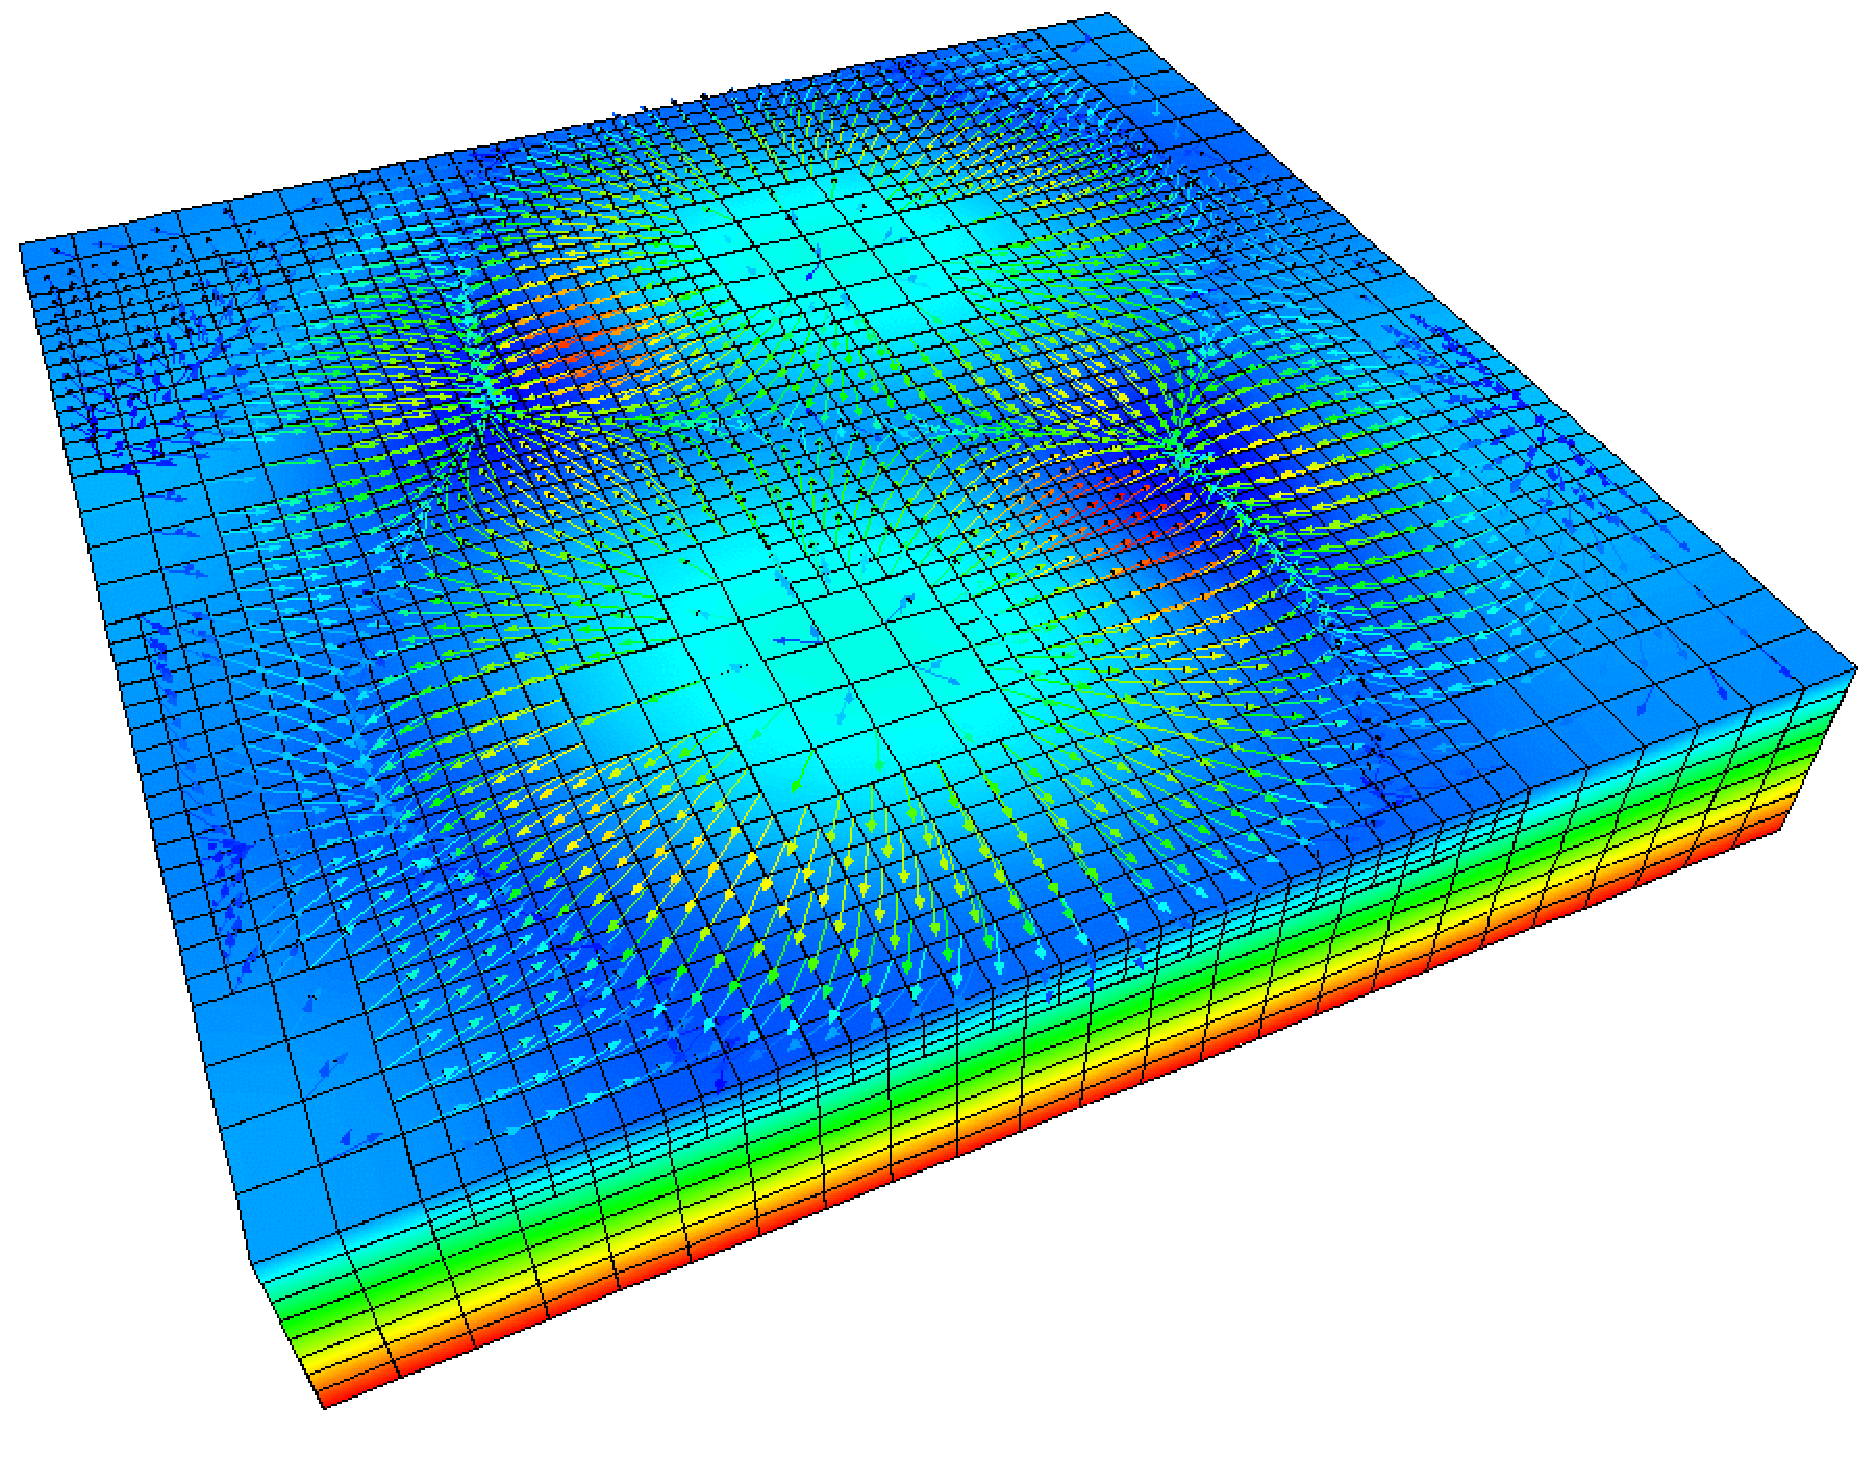
\includegraphics[width=.6\textwidth]{figures/rbm_adapt_soln}    
%%   \end{center}
%%   \vspace{-.25in}

%% %  \begin{block}{}
%%     \begin{itemize}
%%     \item{Adaptive grid solution shown
%%       with temperature contours and velocity vectors.      }
%%       \end{itemize}
%% %  \end{block}
%% \end{frame}








% Original movie inclusion code from Ben's defense
%\centerline{\includemovie[autoplay,loop,text={\includegraphics[height=.8\textheight]{figures/run2890_computed}}]{}{.8\textheight}{movies/Schlieren_run2890.avi}}



%% \begin{frame}
%%   % FIXME: place-holder image for when movie isn't playing?
%%   % setting height=.8\textwidth shrinks the whole movie
%%   % Does the ``poster'' option work?
%%   % Without an image in the text= argument, the movie is the size of the text ...
%%   % Without any text or image and no sizes given, the size is 0x0 ...
%%   % Options are \includemovie{width}{height}{filename}
%%   \centerline
%%       {
%%         \includemovie[autoplay,loop,text={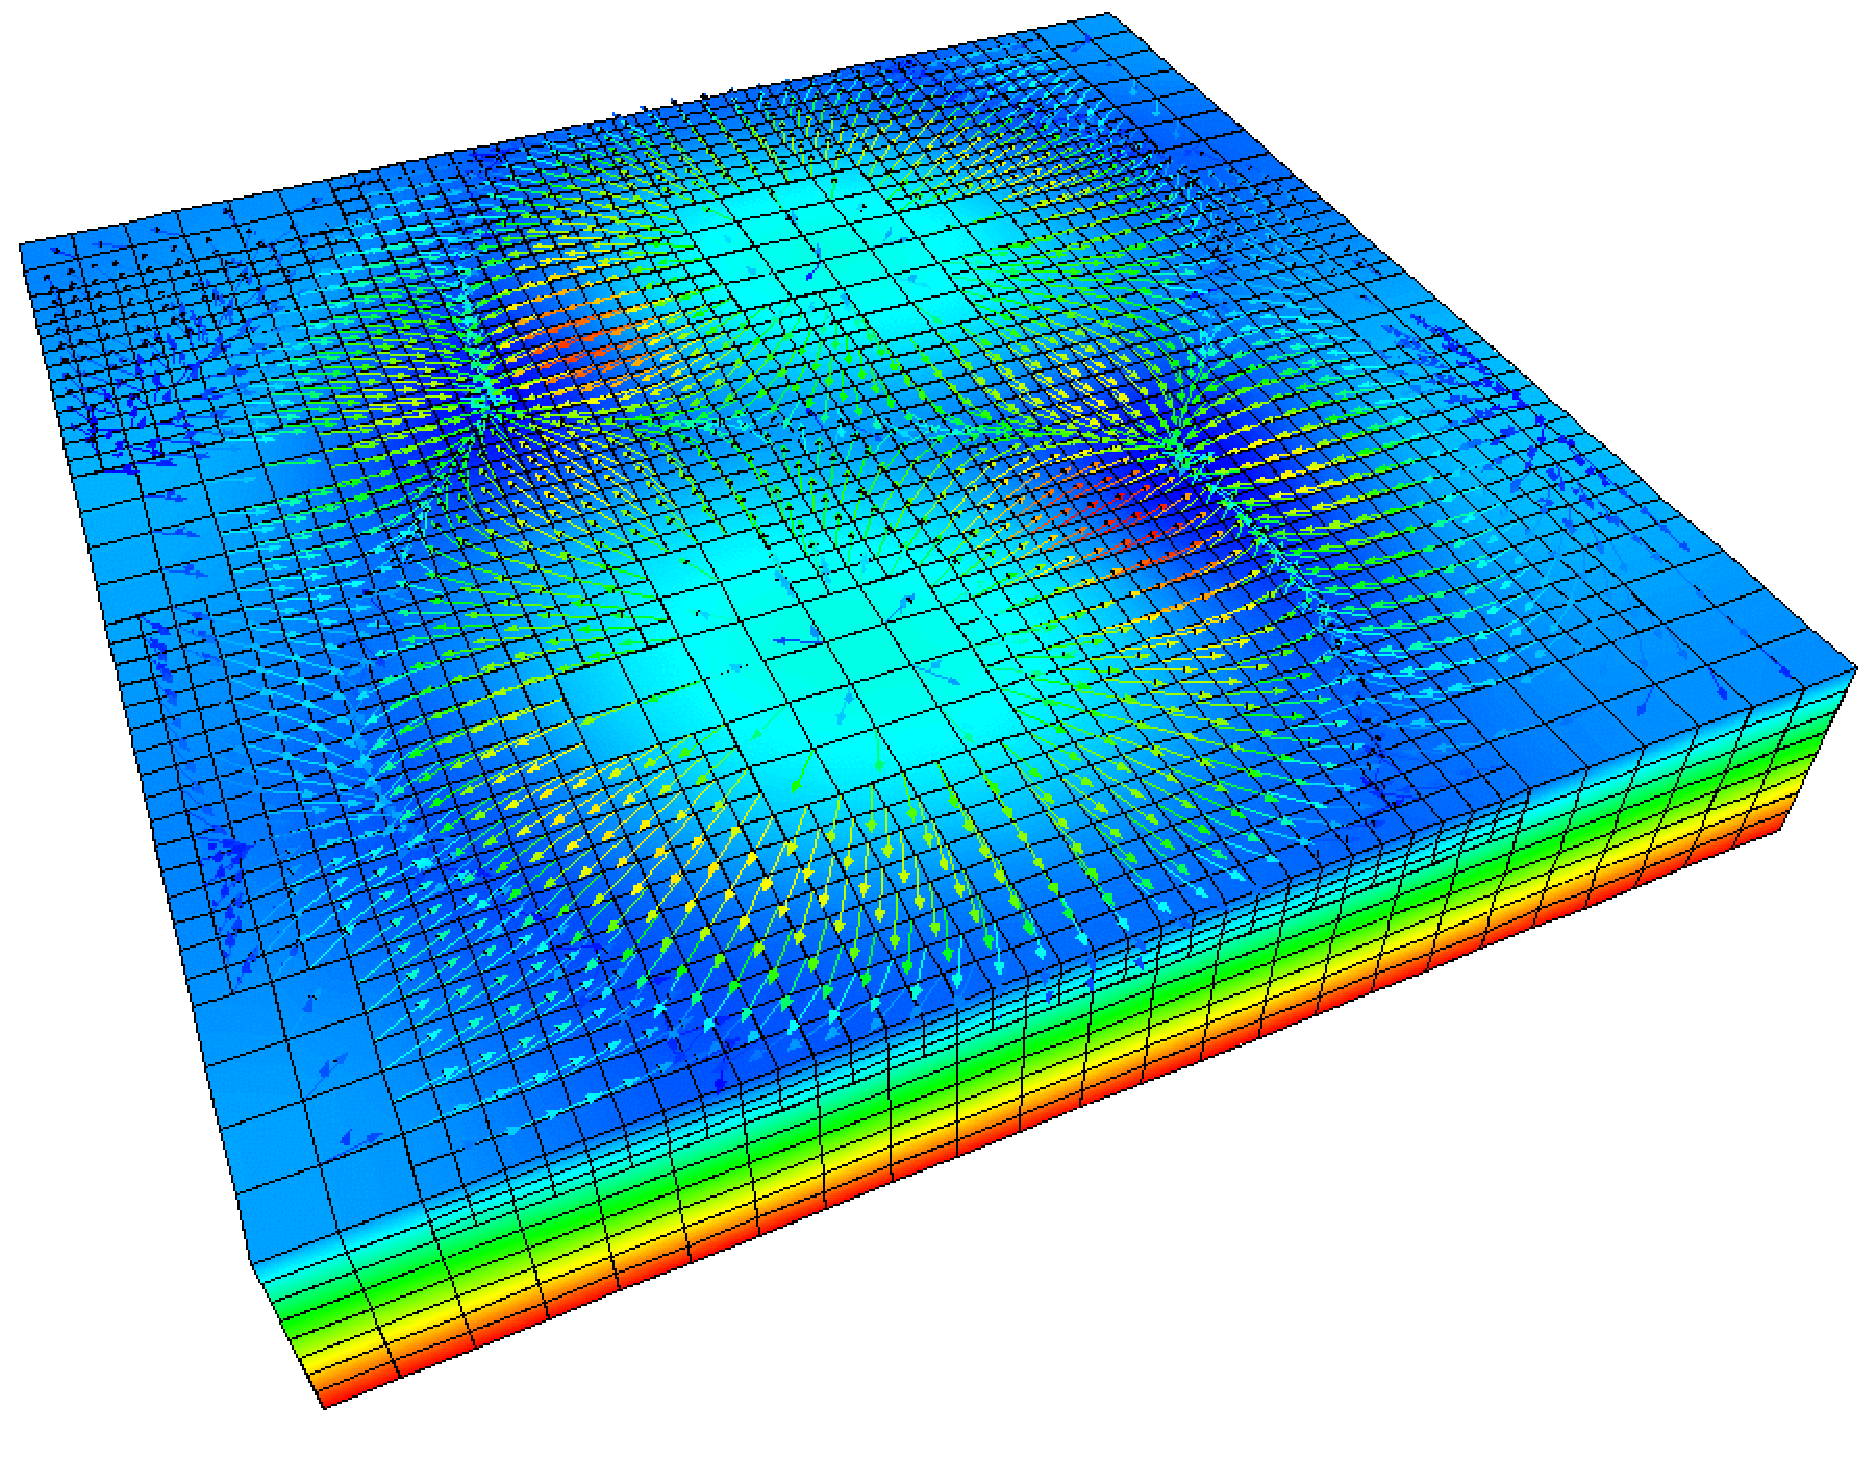
\includegraphics[width=.9\textwidth]{figures/rbm_adapt_soln}}]
%%                      {}{}{movies/Gamma_8_umovie_30x30.avi}
%%       }
%% \end{frame}
